\documentclass[aspectratio=169,t]{beamer}
\usepackage[utf8]{inputenc}
\usepackage[T1]{fontenc}
\usepackage[export]{adjustbox}
\usepackage{threeparttable}
\usepackage{hyperref}
\usepackage{listings}
\usepackage{xcolor}
\usepackage{mdframed}
\usepackage{caption}


\title{Ausgewählte Kapitel der Gesundheitsinformatik}
\date{WS 2019/2020}
\author[PWD]{Prof. Dr.-Ing. Piotr Wojciech Dabrowski}

\usepackage{HTWBeamerTemplate/beamerthemeHTW}
\addbibresource{Bilder/imagesources.bib}
\begin{document}

\setbeamertemplate{background}[bgfirst]
\setbeamertemplate{footline}[first]
\subtitle{Bioinformatik}
\titlegraphic{Bilder/saelogo.jpg}
\begin{frame}[noframenumbering]
    \titlepage
    \begin{textblock}{10}(4.75,15)
    \cite{saelogo}
    \end{textblock}
\end{frame}
\setbeamertemplate{footline}[presentationbody] 
\setbeamertemplate{background}[bgbody]

\begin{frame}{Vorstellung}
    \note<4->{
        Erstes Mal Vorlesung an der HTW\\Bitte um Geduld, Hinweise\\
        \begin{itemize}
            \item Lerne erst Modalitäten kennen
            \item Kenne die Vorkenntnisse/präferierte Art der Studierenden nicht
            \item Primäres Ziel: Verständnis aufbauen, "durch den Stoff kommen" zweitrangig
            \item Also bitte (rechtzeitig) melden, wenn Interesse an Vertiefung besteht
            \item Gemeinsame Reise - bitte immer melden, wenn was ist!
            \item Gerne auch außerhalb der Sprechzeiten, wenn die Tür offen ist einfach reinkommen.
        \end{itemize}
        Whiteboard:
        \begin{itemize}
            \item Wer nicht aufgerufen werden will, nach der VL bei mir melden (stelle keine Fragen) oder X oben links bei Antwort
            \item Spontanes, prägnantes, kohärentes Sprechen wichtig! Beispiel: Empfehlung an Politikerin
        \end{itemize}
    }
    \begin{itemize}
        \item<2-> Kurz zu mir
        \only<2-5>{
            \begin{itemize}
                \item<2-5> Kontakt: Piotr.Dabrowski@htw-berlin.de, Sprechstunde Montag 10-11 - gerne nutzen!
                \item<2-5> Github: https://github.com/dabrowskiw/
                \item<3-5> Geboren 1981 in Warschau
                \item<3-5> Studium der Biotechnologie \& Informatik an der TU Berlin
                \item<3-5> Promotion über Auswertung von Hochdurchsatzdaten für Virus-Diagnostik
                \item<3-5> Aufbau der bioinformatischen Analytik für das NGS-Labor des RKI
                \item<3-5> Aufbau der Bioinformatics Core Facility am RKI
                \item<4-5> Seit WS 2019/2020 an der HTW
                \item<5> Hang zum Experimentieren in der Vorlesung Feedback erwünscht!
            \end{itemize}
        }
        \item<6-> Der Todesstern \& Mini-Whiteboards
    \end{itemize}
\end{frame}


\begin{frame}{Allgemeine Einführung}
     \begin{textblock}{9.2}(1,3)
         \begin{mdframed}[backgroundcolor=white]
            \begin{center}
                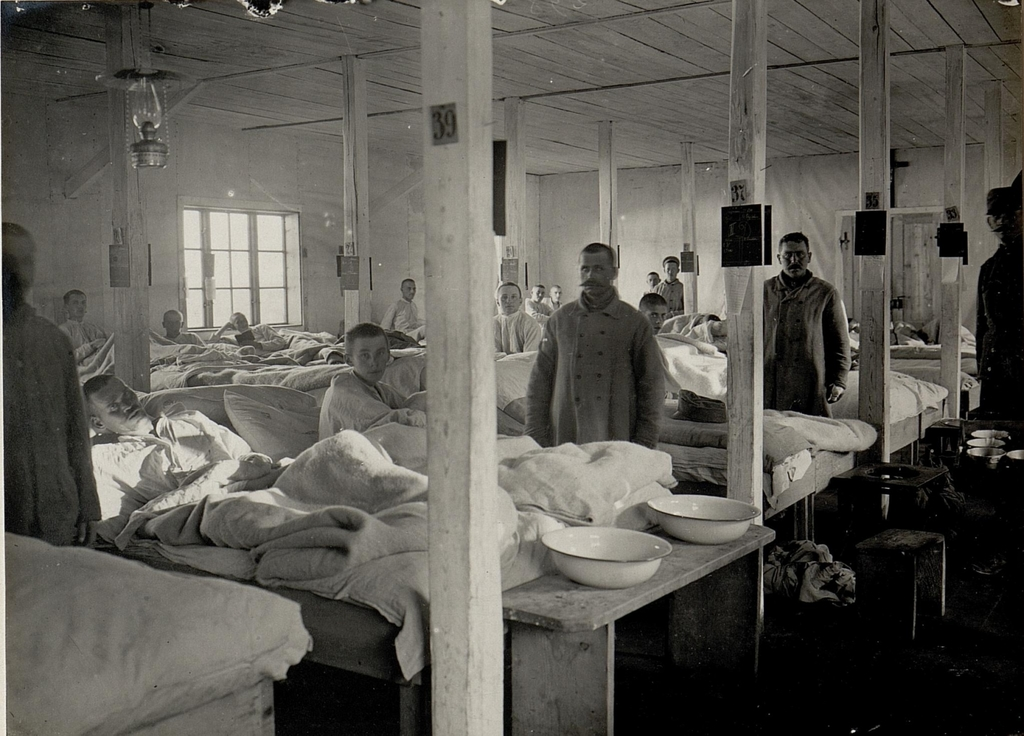
\includegraphics[height=5.3cm]{Bilder/typhus_illness.jpg}\\
                \vspace{0.3cm}\captionof{figure}{Typhuszimmer 1916 \cite{typhus_illness}}
            \end{center}
        \end{mdframed}
    \end{textblock}
    \only<2->{
        \begin{textblock}{9.2}(2,3.1)
            \begin{mdframed}[backgroundcolor=white]
                \begin{center}
                    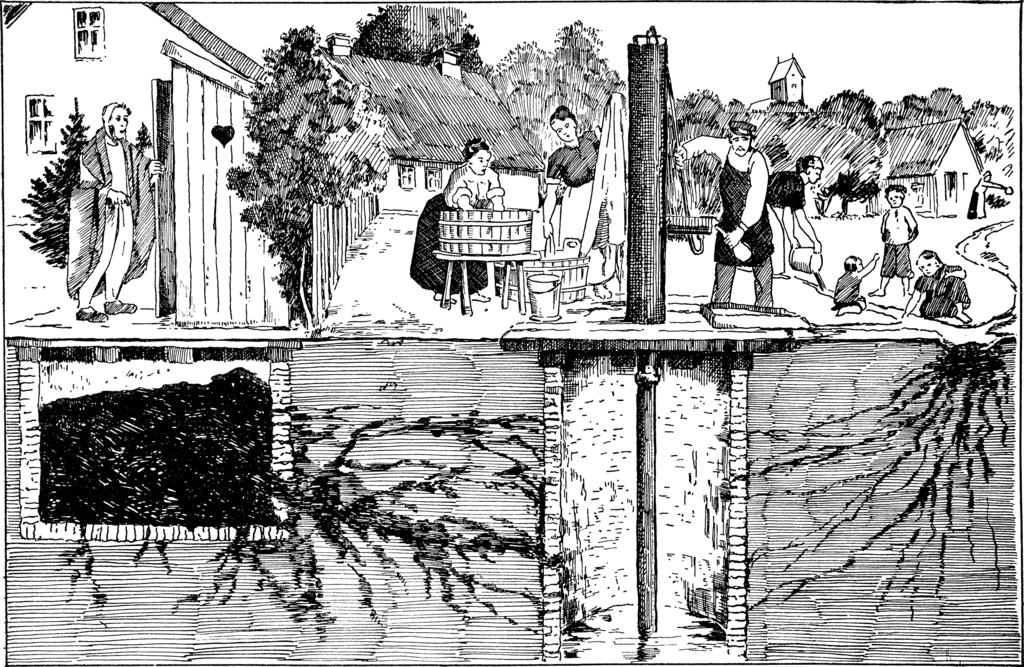
\includegraphics[height=5.3cm]{Bilder/typhus_spread.png}\\
                    \vspace{0.3cm}\captionof{figure}{Visualisierung der Typhusverbreitung in einem Buch von 1939 \cite{typhus_spread}}
                \end{center}
            \end{mdframed}
        \end{textblock}
    }
    \only<3->{
        \begin{textblock}{9.2}(3,3.2)
            \begin{mdframed}[backgroundcolor=white]
                \begin{center}
                    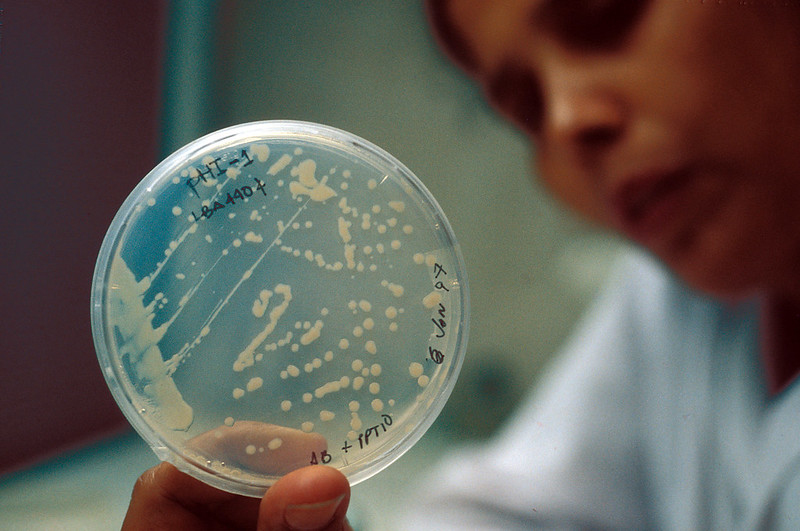
\includegraphics[height=5.3cm]{Bilder/typhus_petri.jpg}\\
                    \vspace{0.3cm}\captionof{figure}{Bakterienkulturen in einer Petrischale \cite{typhus_petri}}
                \end{center}
            \end{mdframed}
        \end{textblock}
    }
    \only<4->{
        \begin{textblock}{9.2}(4,3.3)
            \begin{mdframed}[backgroundcolor=white]
                \begin{center}
                    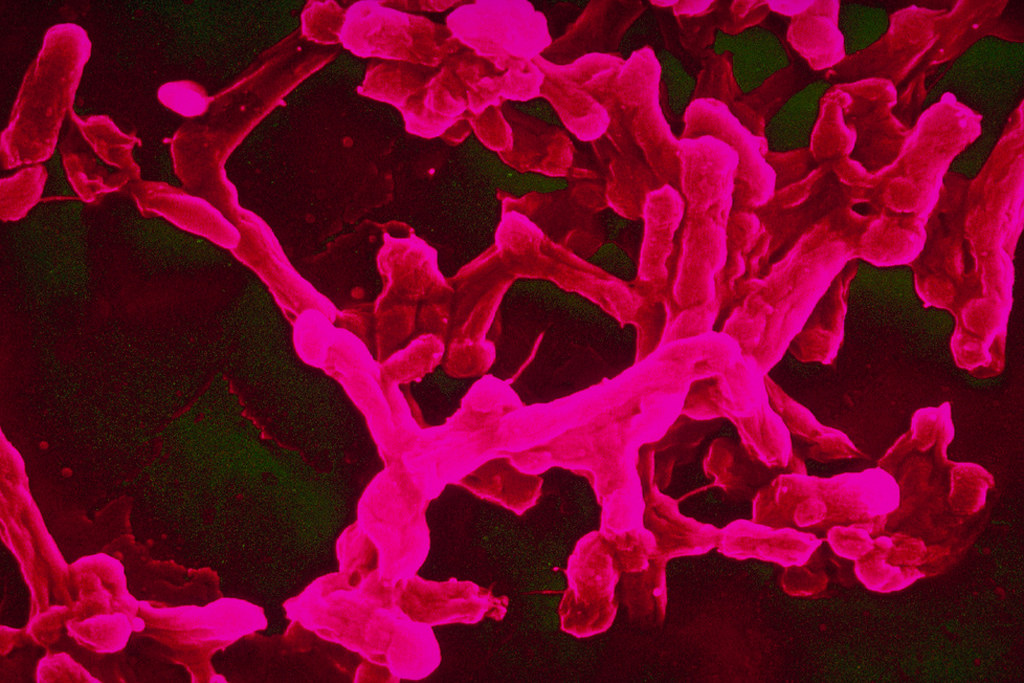
\includegraphics[height=5.3cm]{Bilder/typhus_em.jpg}\\
                    \vspace{0.3cm}\captionof{figure}{Elektronenmikroskopische Aufnahme von Typhus-Bakterien \cite{typhus_em}}
                \end{center}
            \end{mdframed}
        \end{textblock}
    }
    \only<5->{
        \begin{textblock}{9.2}(5,3.4)
            \begin{mdframed}[backgroundcolor=white]
                \begin{center}
                    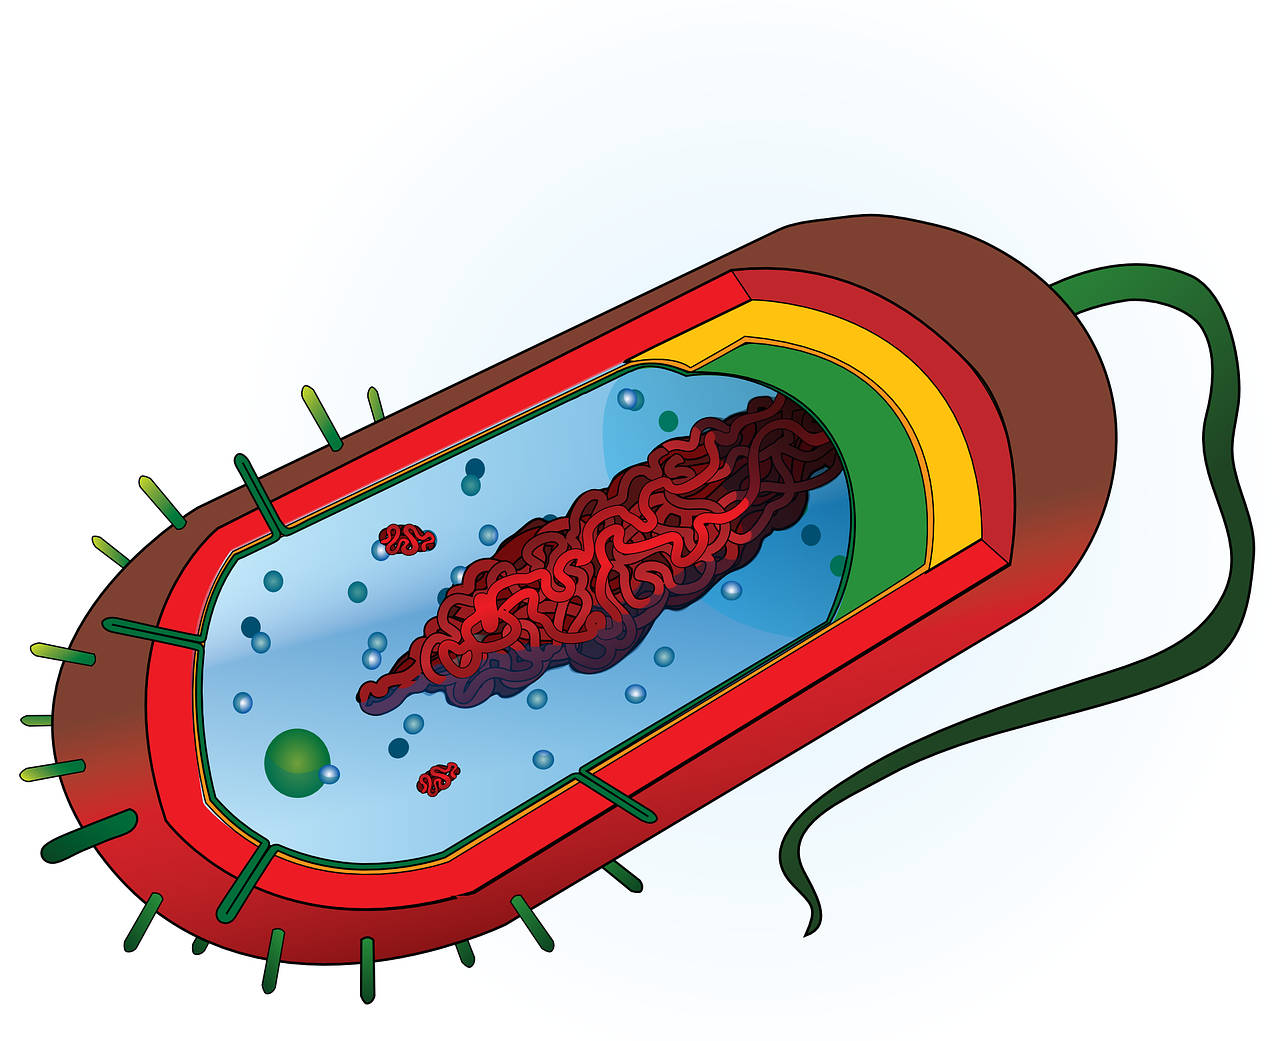
\includegraphics[height=5.3cm]{Bilder/bacterium.jpg}\\
                    \vspace{0.3cm}\captionof{figure}{Schematische Darstellung eins Bakteriums \cite{bacterium}}
                \end{center}
            \end{mdframed}
        \end{textblock}
    }
    \only<6->{
        \begin{textblock}{9.2}(6,3.5)
            \begin{mdframed}[backgroundcolor=white]
                \begin{center}
                    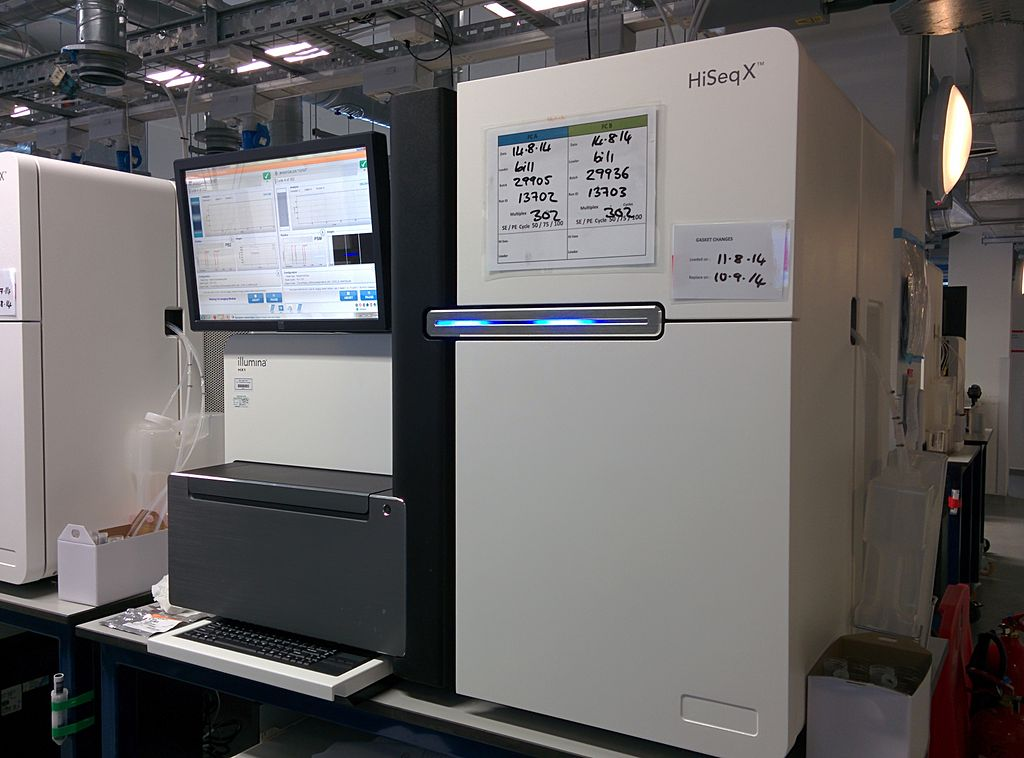
\includegraphics[height=5.3cm]{Bilder/hiseq.jpg}\\
                    \vspace{0.3cm}\captionof{figure}{Ein aktuelles Next Generation Sequencing-Gerät \cite{hiseq}}
                \end{center}
            \end{mdframed}
        \end{textblock}
    }
\end{frame}

\begin{frame}{Die Herausforderung}
    \only<1->{
        \begin{textblock}{9.2}(1,3)
            \begin{mdframed}[backgroundcolor=white]
                \begin{center}
                    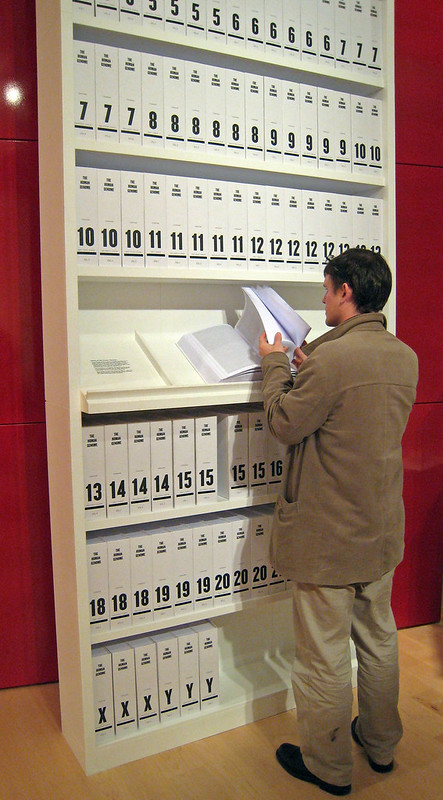
\includegraphics[height=5.2cm]{Bilder/problem1.jpg}\\
                    \vspace{0.3cm}\captionof{figure}{Das humane Genom ausgedruckt\cite{problem1}}
                \end{center}
            \end{mdframed}
        \end{textblock}
    }
    \only<2->{
        \begin{textblock}{9.2}(2,3.1)
            \begin{mdframed}[backgroundcolor=white]
                \begin{center}
                    
\includegraphics[height=5.2cm]{Bilder/problem2.jpg}\\
                    \vspace{0.3cm}\captionof{figure}{Ein Comic-Heft als Veranschaulichung des Größenverhältnisses von humanem zu Krankenerreger-Genom\cite{problem2}}
                \end{center}
            \end{mdframed}
        \end{textblock}
    }
    \only<3->{
        \begin{textblock}{9.2}(3,3.2)
            \begin{mdframed}[backgroundcolor=white]
                \begin{center}
                    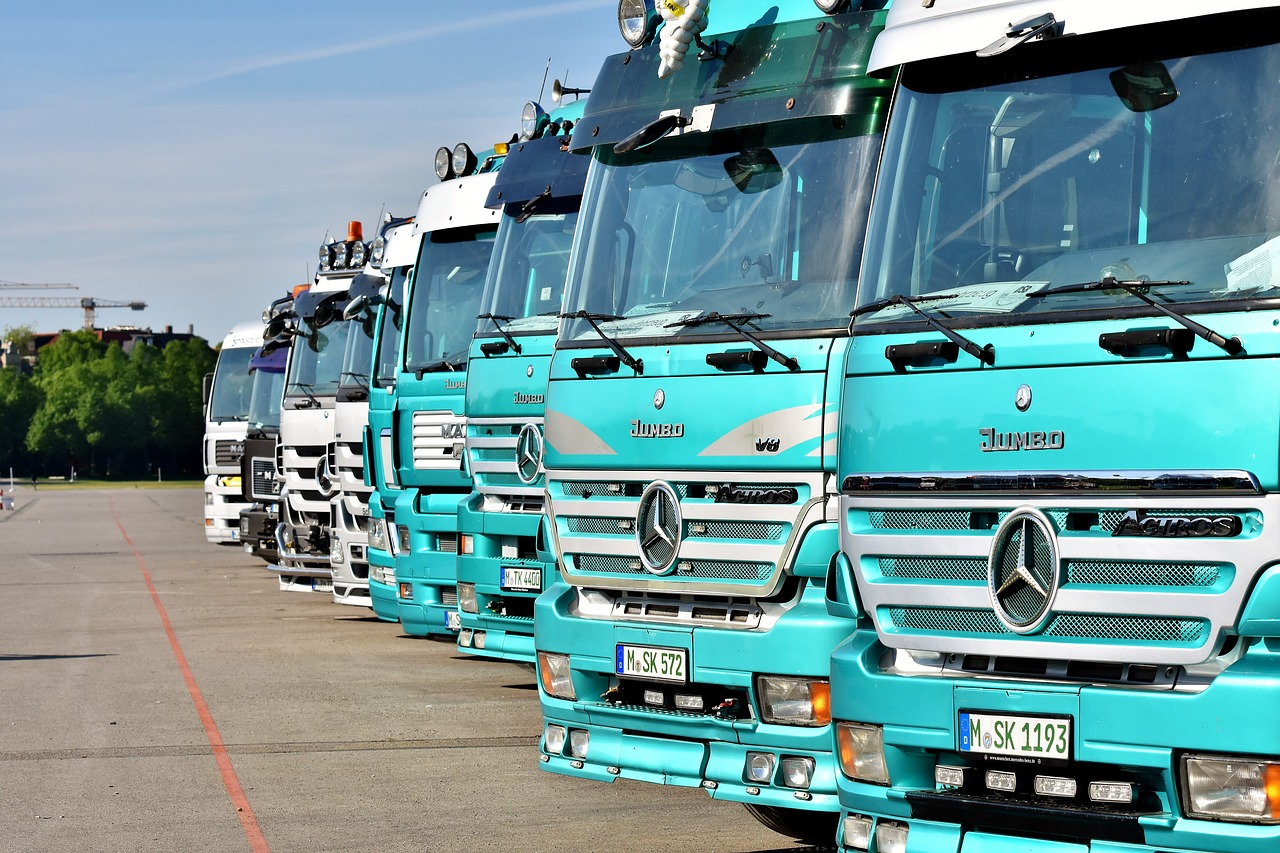
\includegraphics[height=5.2cm]{Bilder/problem3.jpg}\\
                    \vspace{0.3cm}\captionof{figure}{LKW-Flotte - das bräuchte man, um die ausgedruckten Sequenzen eines NGS-Laufes zu transportieren\cite{problem3}}
                \end{center}
            \end{mdframed}
        \end{textblock}
    }
    \only<4->{
        \begin{textblock}{9.2}(4,3.3)
            \begin{mdframed}[backgroundcolor=white]
                \begin{center}
                    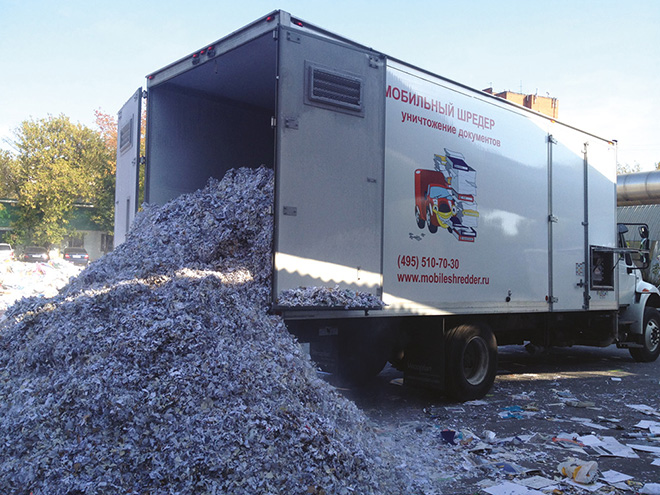
\includegraphics[height=5.2cm]{Bilder/problem4.jpg}\\
                    \vspace{0.3cm}\captionof{figure}{Industrieschredder - das, was beim Next Generation Sequencing mit dem Genom passiert \cite{problem4}}
                \end{center}
            \end{mdframed}
        \end{textblock}
    }
    \only<5->{
        \begin{textblock}{10}(5,3.4)
            \begin{mdframed}[backgroundcolor=white]
                \begin{center}
                    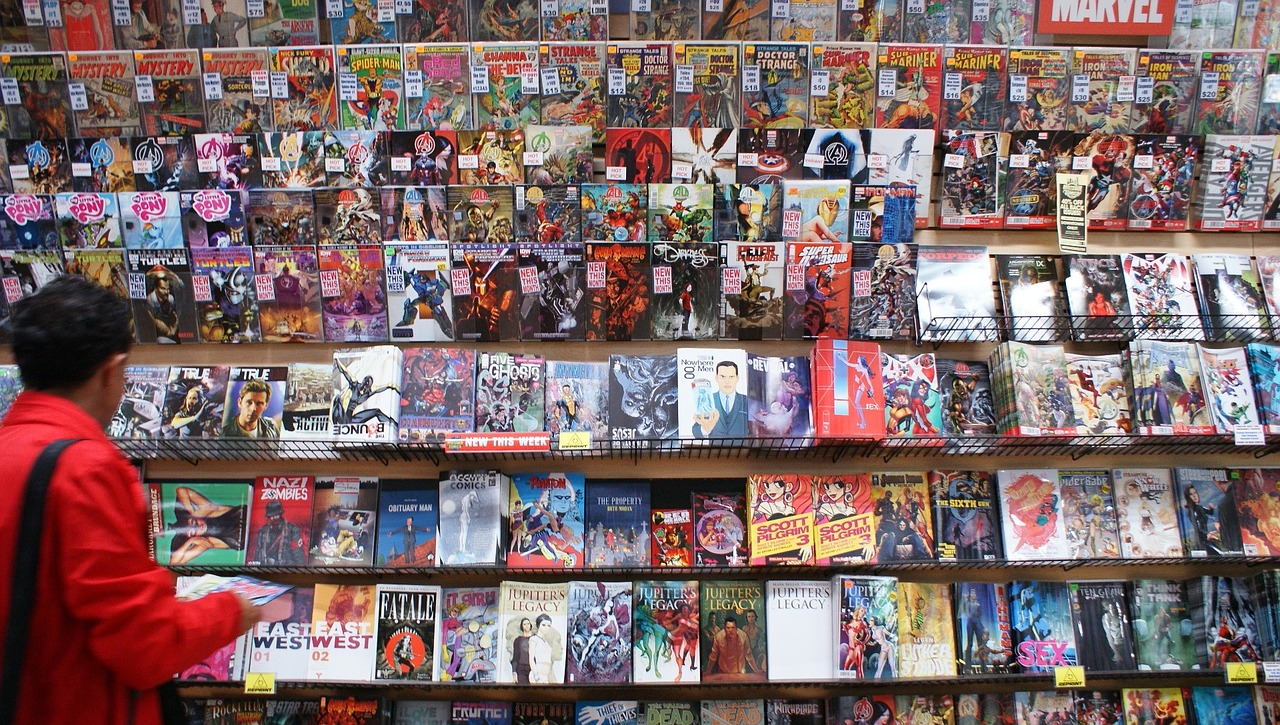
\includegraphics[height=5.2cm]{Bilder/problem5.jpg}\\
                    \vspace{0.3cm}\captionof{figure}{Krankheitserreger sind noch vielfältiger als Comic-Hefte\cite{problem5}}
                \end{center}
            \end{mdframed}
        \end{textblock}
    }
\end{frame}

\begin{frame}[allowframebreaks]{Quellenangaben}
    \printbibliography
\end{frame}

\begin{frame}{Lizenz}
    \begin{center}
        
\includegraphics{Bilder/by.png}\\
        Alle Inhalte außer dem HTW-Logo, für die keine Quelle angegeben ist, sind eigenes Material und unter CC-BY 4.0\\
        \url{https://creativecommons.org/licenses/by/4.0/}\\
        lizenziert.\\\vspace{0.5cm}
        Sämtliche Nutzungs- und Verwertungsrechte für das Logo der HTW Berlin in allen hier verwendeten Formen liegen ausschließlich bei der HTW Berlin:\\
        \url{https://corporatedesign.htw-berlin.de/logos/logo-htw-berlin/}
    \end{center}
\end{frame}

\end{document}